%Se deben explicar todas las pruebas de sintonización manual realizadas. Para esto debe usar la estructura que se adjunta abajo.\\

Para la presente sección, se requiere de una configuración inicial,
para poder comenzar a evaluar el rendimiento del algoritmo para
cada situación donde se quiera sintonizar manualmente algún parámetro.

Los valores de la configuración inicial están dado en base a la experiencia
del trabajo pasado, es decir, en la \emph{primera implementación}.

\begin{itemize}
	\item \texttt{POP = 20}
	\item \texttt{GENS = 200}
	\item \texttt{clonationFactor = 0.4}
	\item \texttt{clonationRate = 0.5}
	\item \texttt{replaceRate = 0.6}
\end{itemize}

Complementariamente, se han considerado tres instancias provenientes de la CSPlib~\cite{CSP}
más precisamente de la sección \emph{``30 new hard problems from Caroline Gagne ''},
donde se han escogido tomando en cuenta el mejor resultado encontrado.
Las instancias son:

\begin{center}
	\begin{tabular}{|l|c|}
	\hline
	\textbf{Instancia} & \textbf{Mejor resultado conocido} \\\hline
	\texttt{pb\_200\_01.txt} & 0 \\\hline
	\texttt{pb\_200\_09.txt} & 10 \\\hline
	\texttt{pb\_200\_10.txt} & 19 \\\hline
	\end{tabular}
\end{center}
\newpage
\subsubsection{Tamaño de población}

\textbf{Prueba}: \blue{prueba1}\\

\textbf{Parámetros involucrados:} Tamaño de población \texttt{(POP)}.\\

\textbf{Objetivo:} Analizar el comportamiento de acuerdo a fitness y tiempo de ejecución del parámetro en un rango de valores.\\

\textbf{Metodología:} Se probarán varios valores en el rango de valores del parámetro \blue{[10,210]}.\\

\textbf{Gráfico:}\\

\begin{figure}[h!]
\begin{center}
	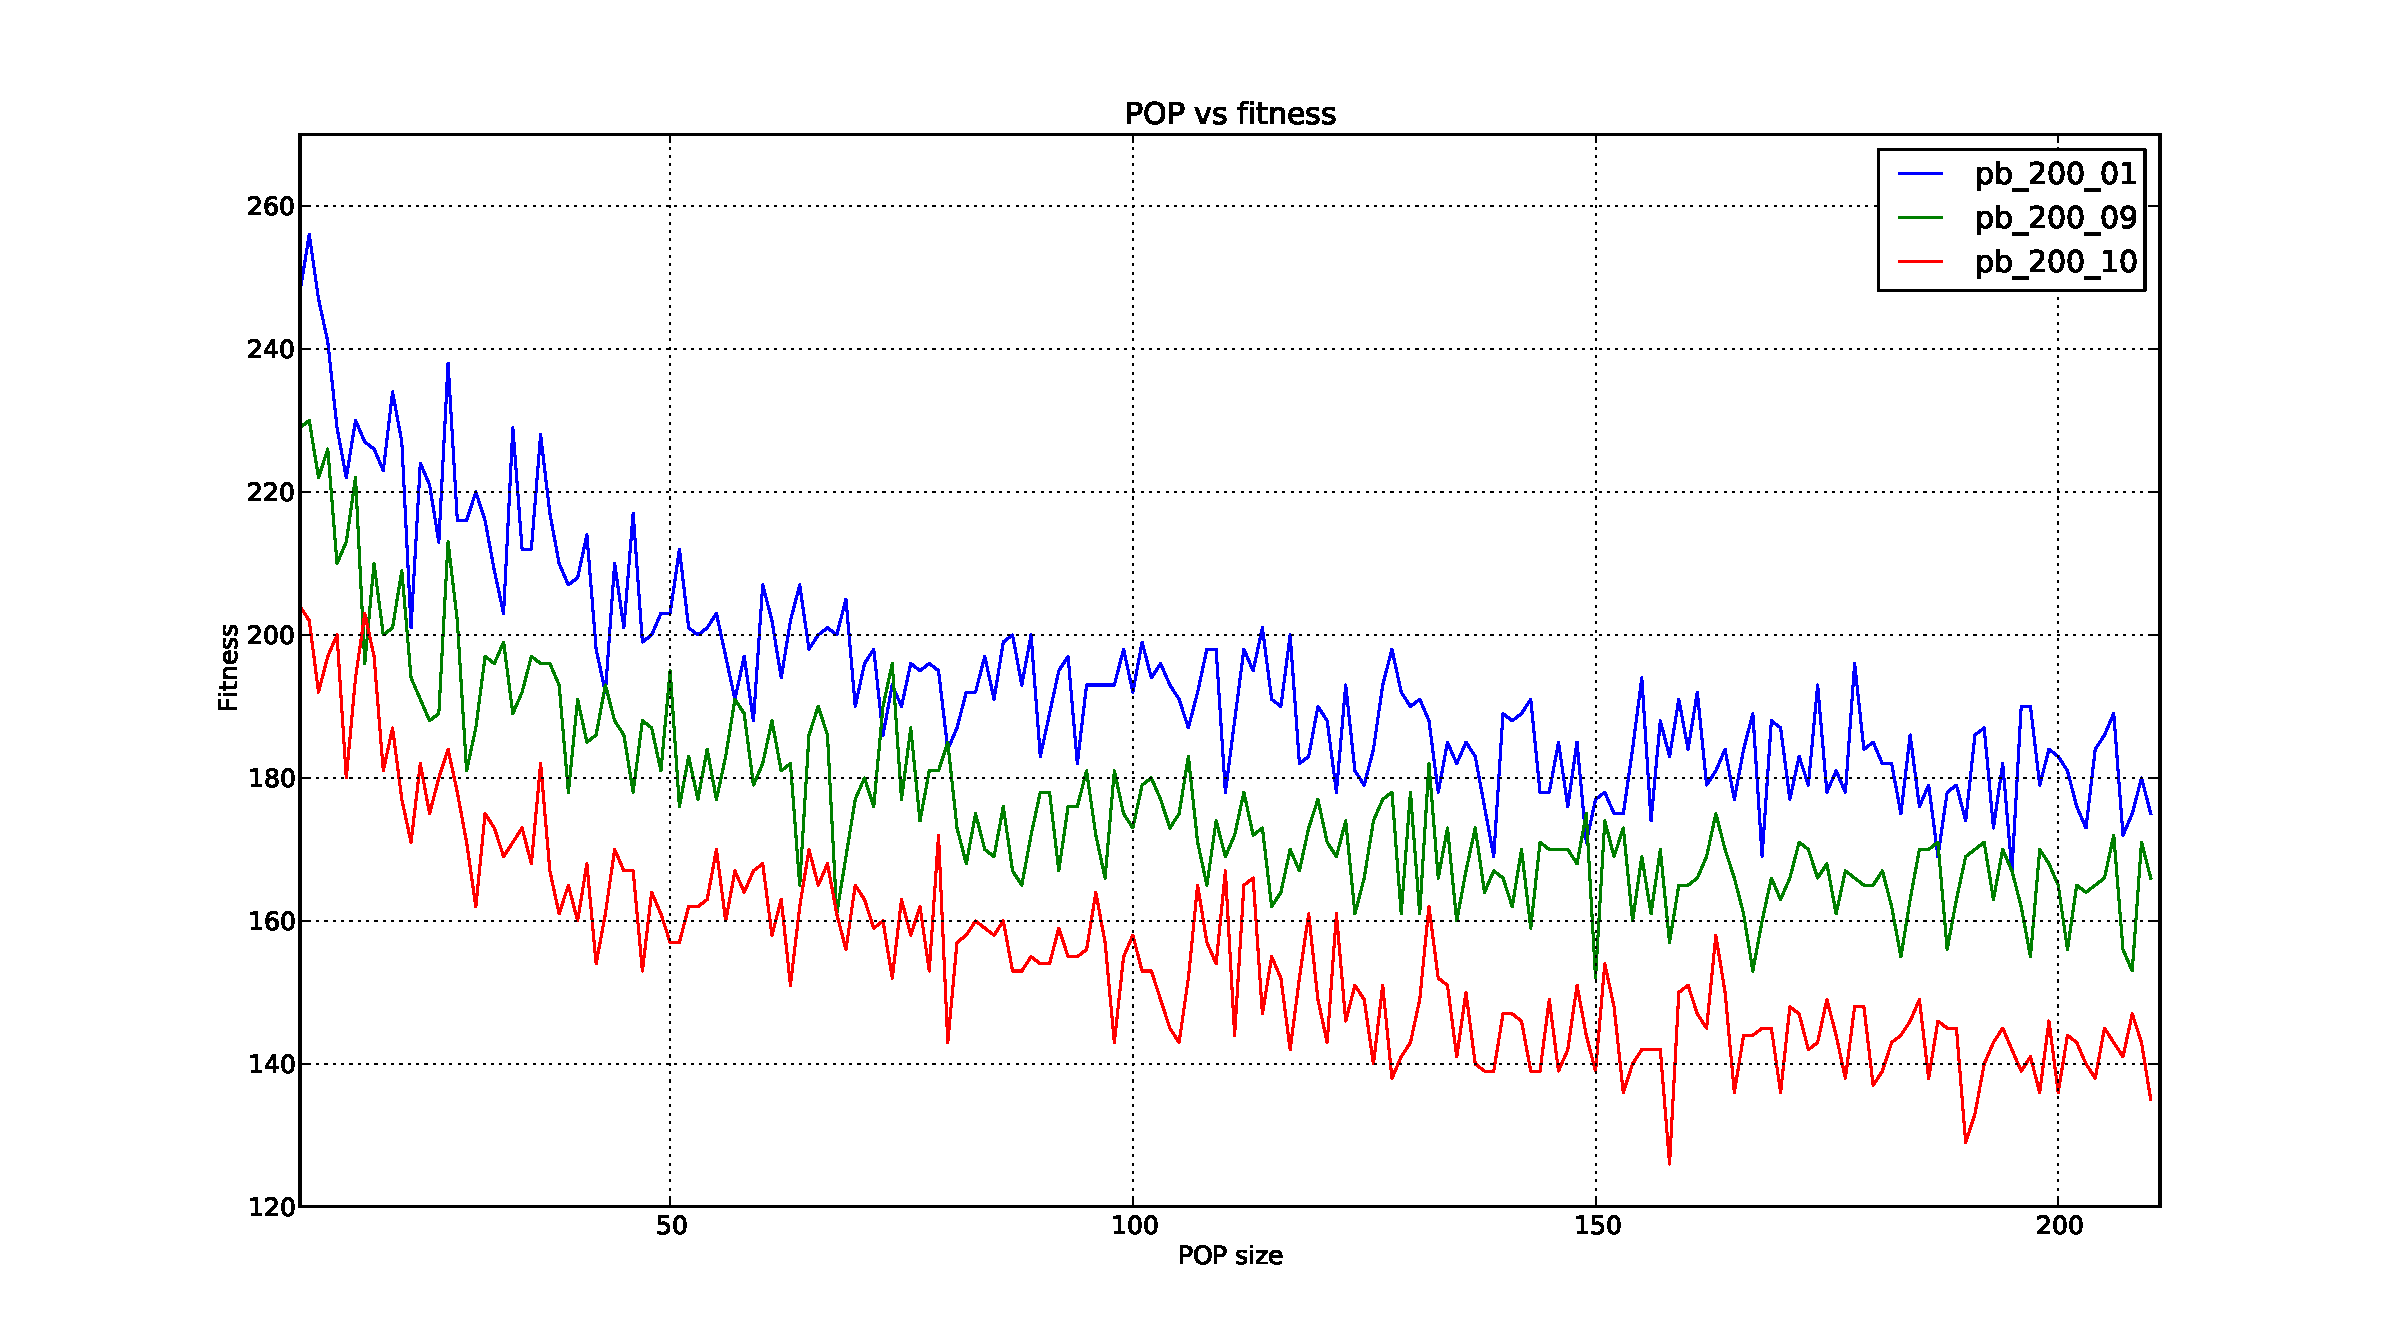
\includegraphics[width=0.95\textwidth]{img/1.pdf}
	\caption{Comparaci\'on de las tres instancias dado un cambio en la poblaci\'on}
	\label{fig:1}
\end{center}
\end{figure}

\textbf{Configuración escogida:}\\

\begin{center}
\begin{tabular}{|l|c|c|c|c|}
	\hline
	\textbf{Instancia} & \textbf{POP} & \textbf{Mejor resultado} & \textbf{Tiempo [s] } & \textbf{Tiempo total [s] }\\\hline
	\texttt{pb\_200\_01.txt} & 195 & 167 & 15.110 & 1608.853 \\\hline 
	\texttt{pb\_200\_09.txt} & 150 & 152 & 11.243 & 1593.739 \\\hline
	\texttt{pb\_200\_10.txt} & 158 & 126 & 11.210 & 1662.580 \\\hline
\end{tabular}
\end{center}

\newpage
\subsubsection{Número de generaciones}

\textbf{Prueba}: \blue{prueba2}\\

\textbf{Parámetros involucrados:} Número de generaciones \texttt{(GENS)}.\\

\textbf{Objetivo:} Analizar el comportamiento de acuerdo a fitness y tiempo de ejecución del número de generaciones entre un rango de valores.\\

\textbf{Metodología:} Se probarán varios valores en el rango de valores del parámetro \blue{[10,2000]} (iterando de 30 en 30).\\

\textbf{Gráfico:}\\

\begin{figure}[h!]
\begin{center}
	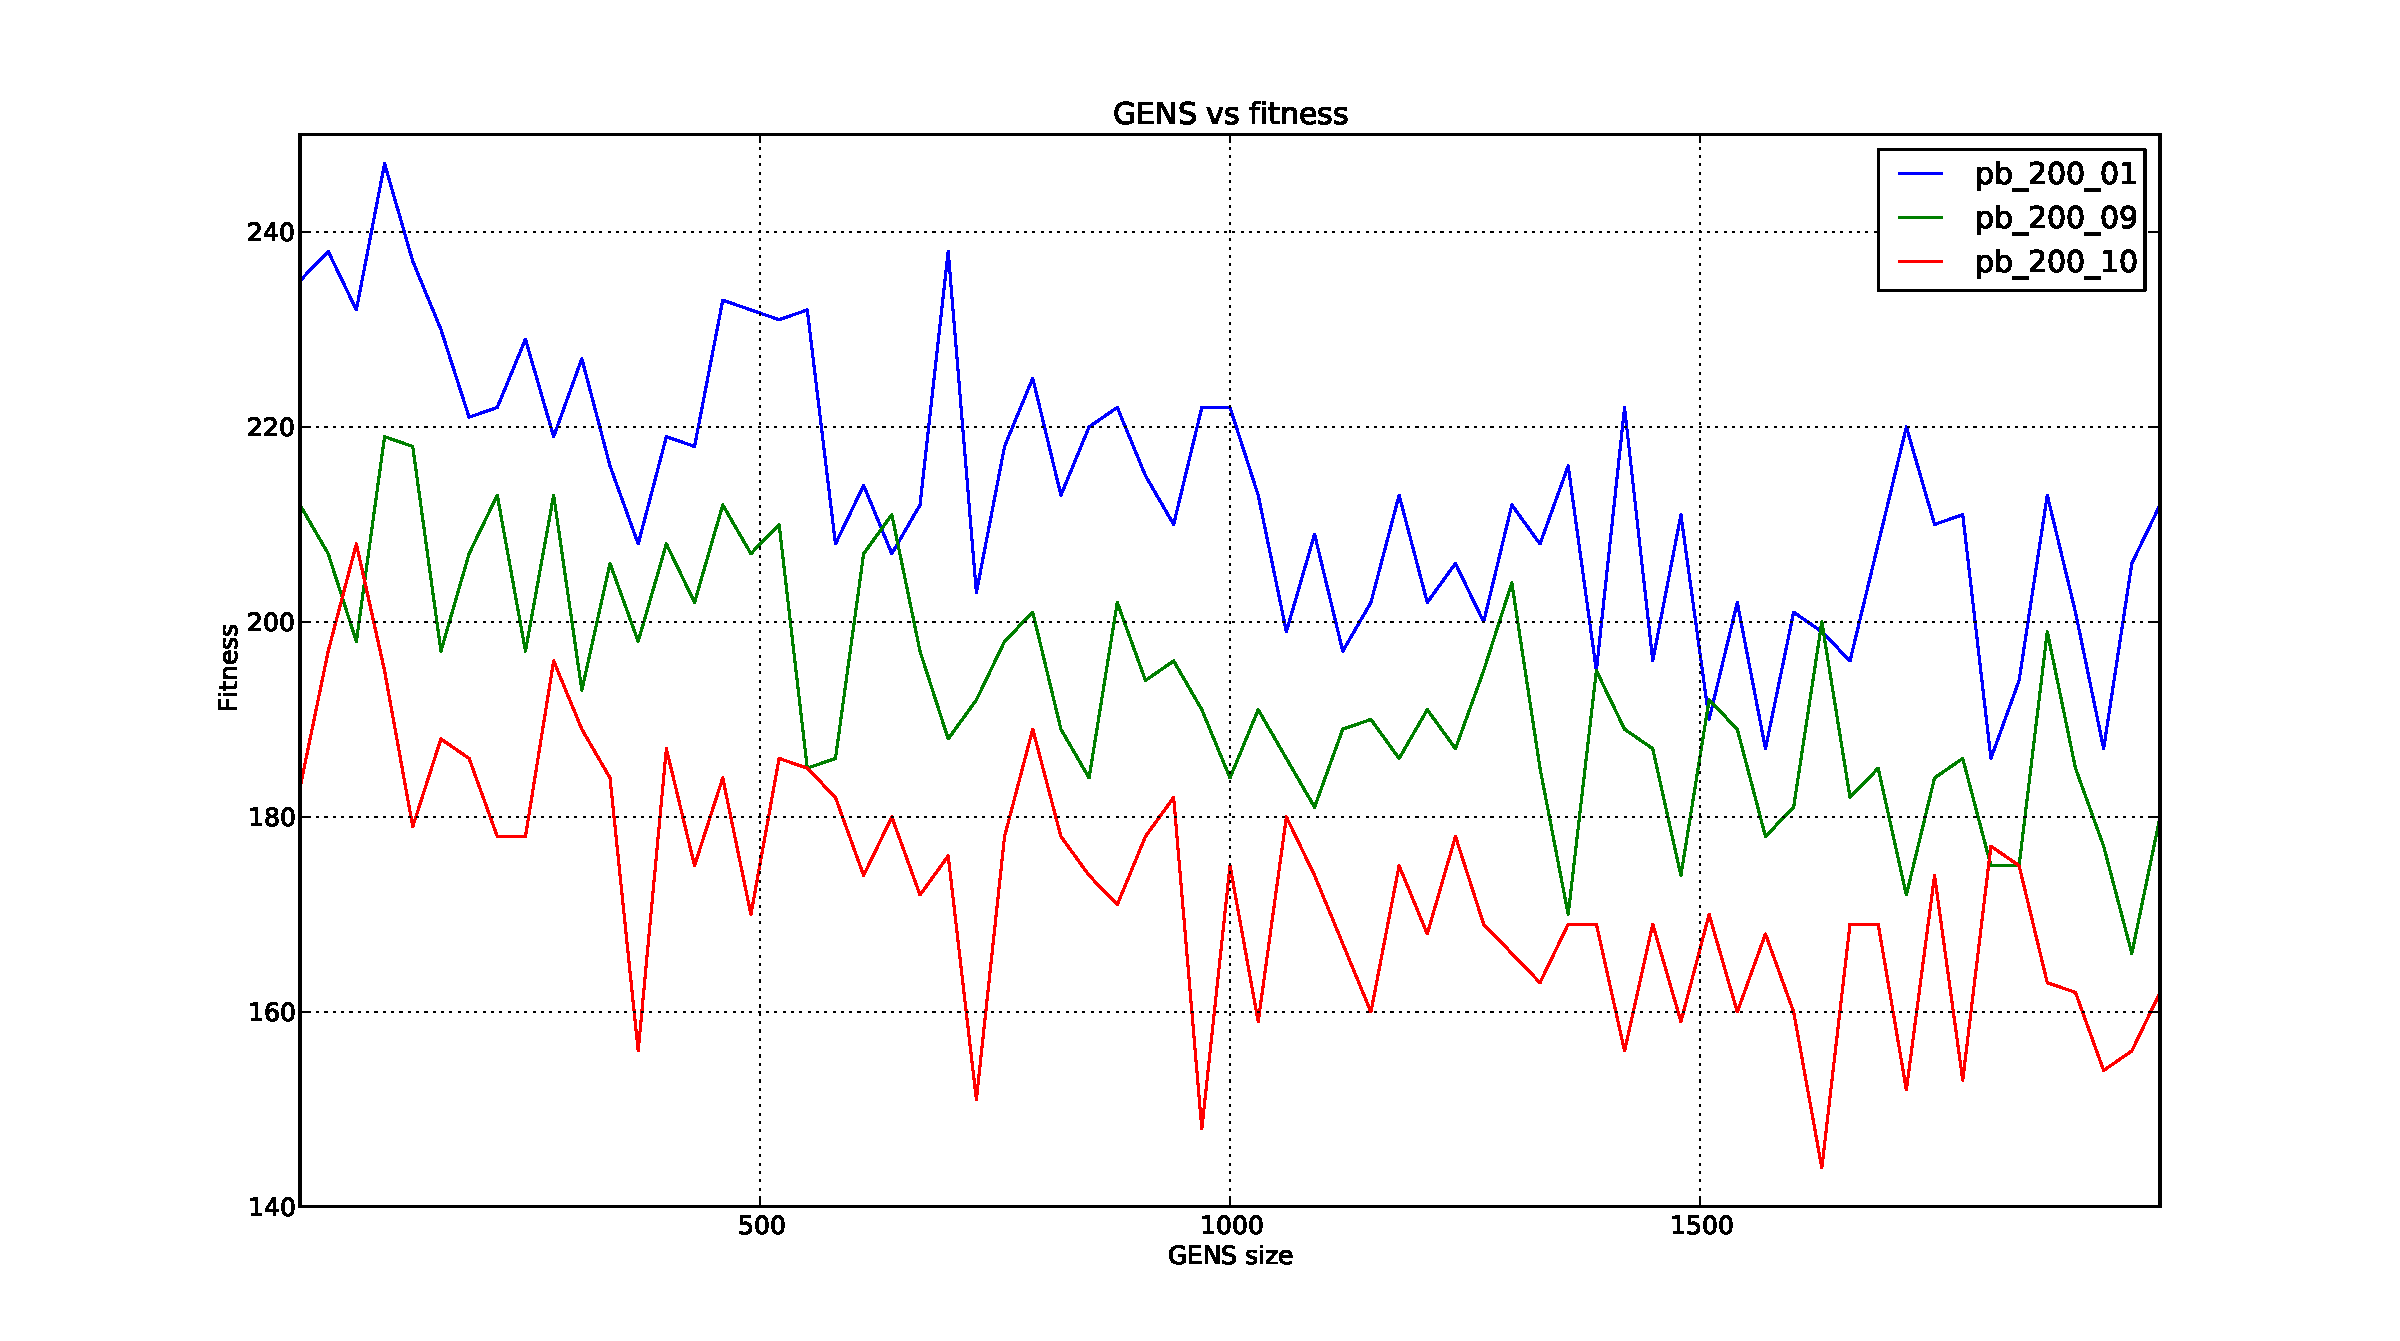
\includegraphics[width=0.95\textwidth]{img/2.pdf}
	\caption{Comparaci\'on de las tres instancias dado un cambio en el n\'umero de generaciones}
	\label{fig:2}
\end{center}
\end{figure}

\textbf{Configuración escogida:}\\

\begin{center}
\begin{tabular}{|l|c|c|c|c|}
	\hline
	\textbf{Instancia} & \textbf{GENS} &\textbf{Mejor resultado} & \textbf{Tiempo [s] } & \textbf{Tiempo total [s]}\\\hline
	\texttt{pb\_200\_01.txt} & 1810 & 186 & 7.782 & 256.177 \\\hline
	\texttt{pb\_200\_09.txt} & 1960 & 166 & 8.460 & 262.906 \\\hline
	\texttt{pb\_200\_10.txt} & 1630 & 144 & 7.562 & 256.546 \\\hline
\end{tabular}
\end{center}

\newpage
\subsubsection{Tasa de reemplazo}

\textbf{Prueba}: \blue{prueba3}\\

\textbf{Parámetros involucrados:} Tasa de reemplazo \texttt{(replaceRate)}.\\

\textbf{Objetivo:} Analizar el comportamiento de acuerdo a fitness y tiempo de ejecución de la tasa de reemplazo entre un rango de valores.\\

\textbf{Metodología:} Se probarán varios valores en el rango de valores del parámetro \blue{[0,1]}.
Para éste caso en particular, se ejecutó el algoritmo 10 veces por cada valor del parámetros y luego se seleccionó la mejor
para poder hacer el siguiente análisis.\\

\textbf{Gráfico:}\\

\begin{figure}[h!]
\begin{center}
	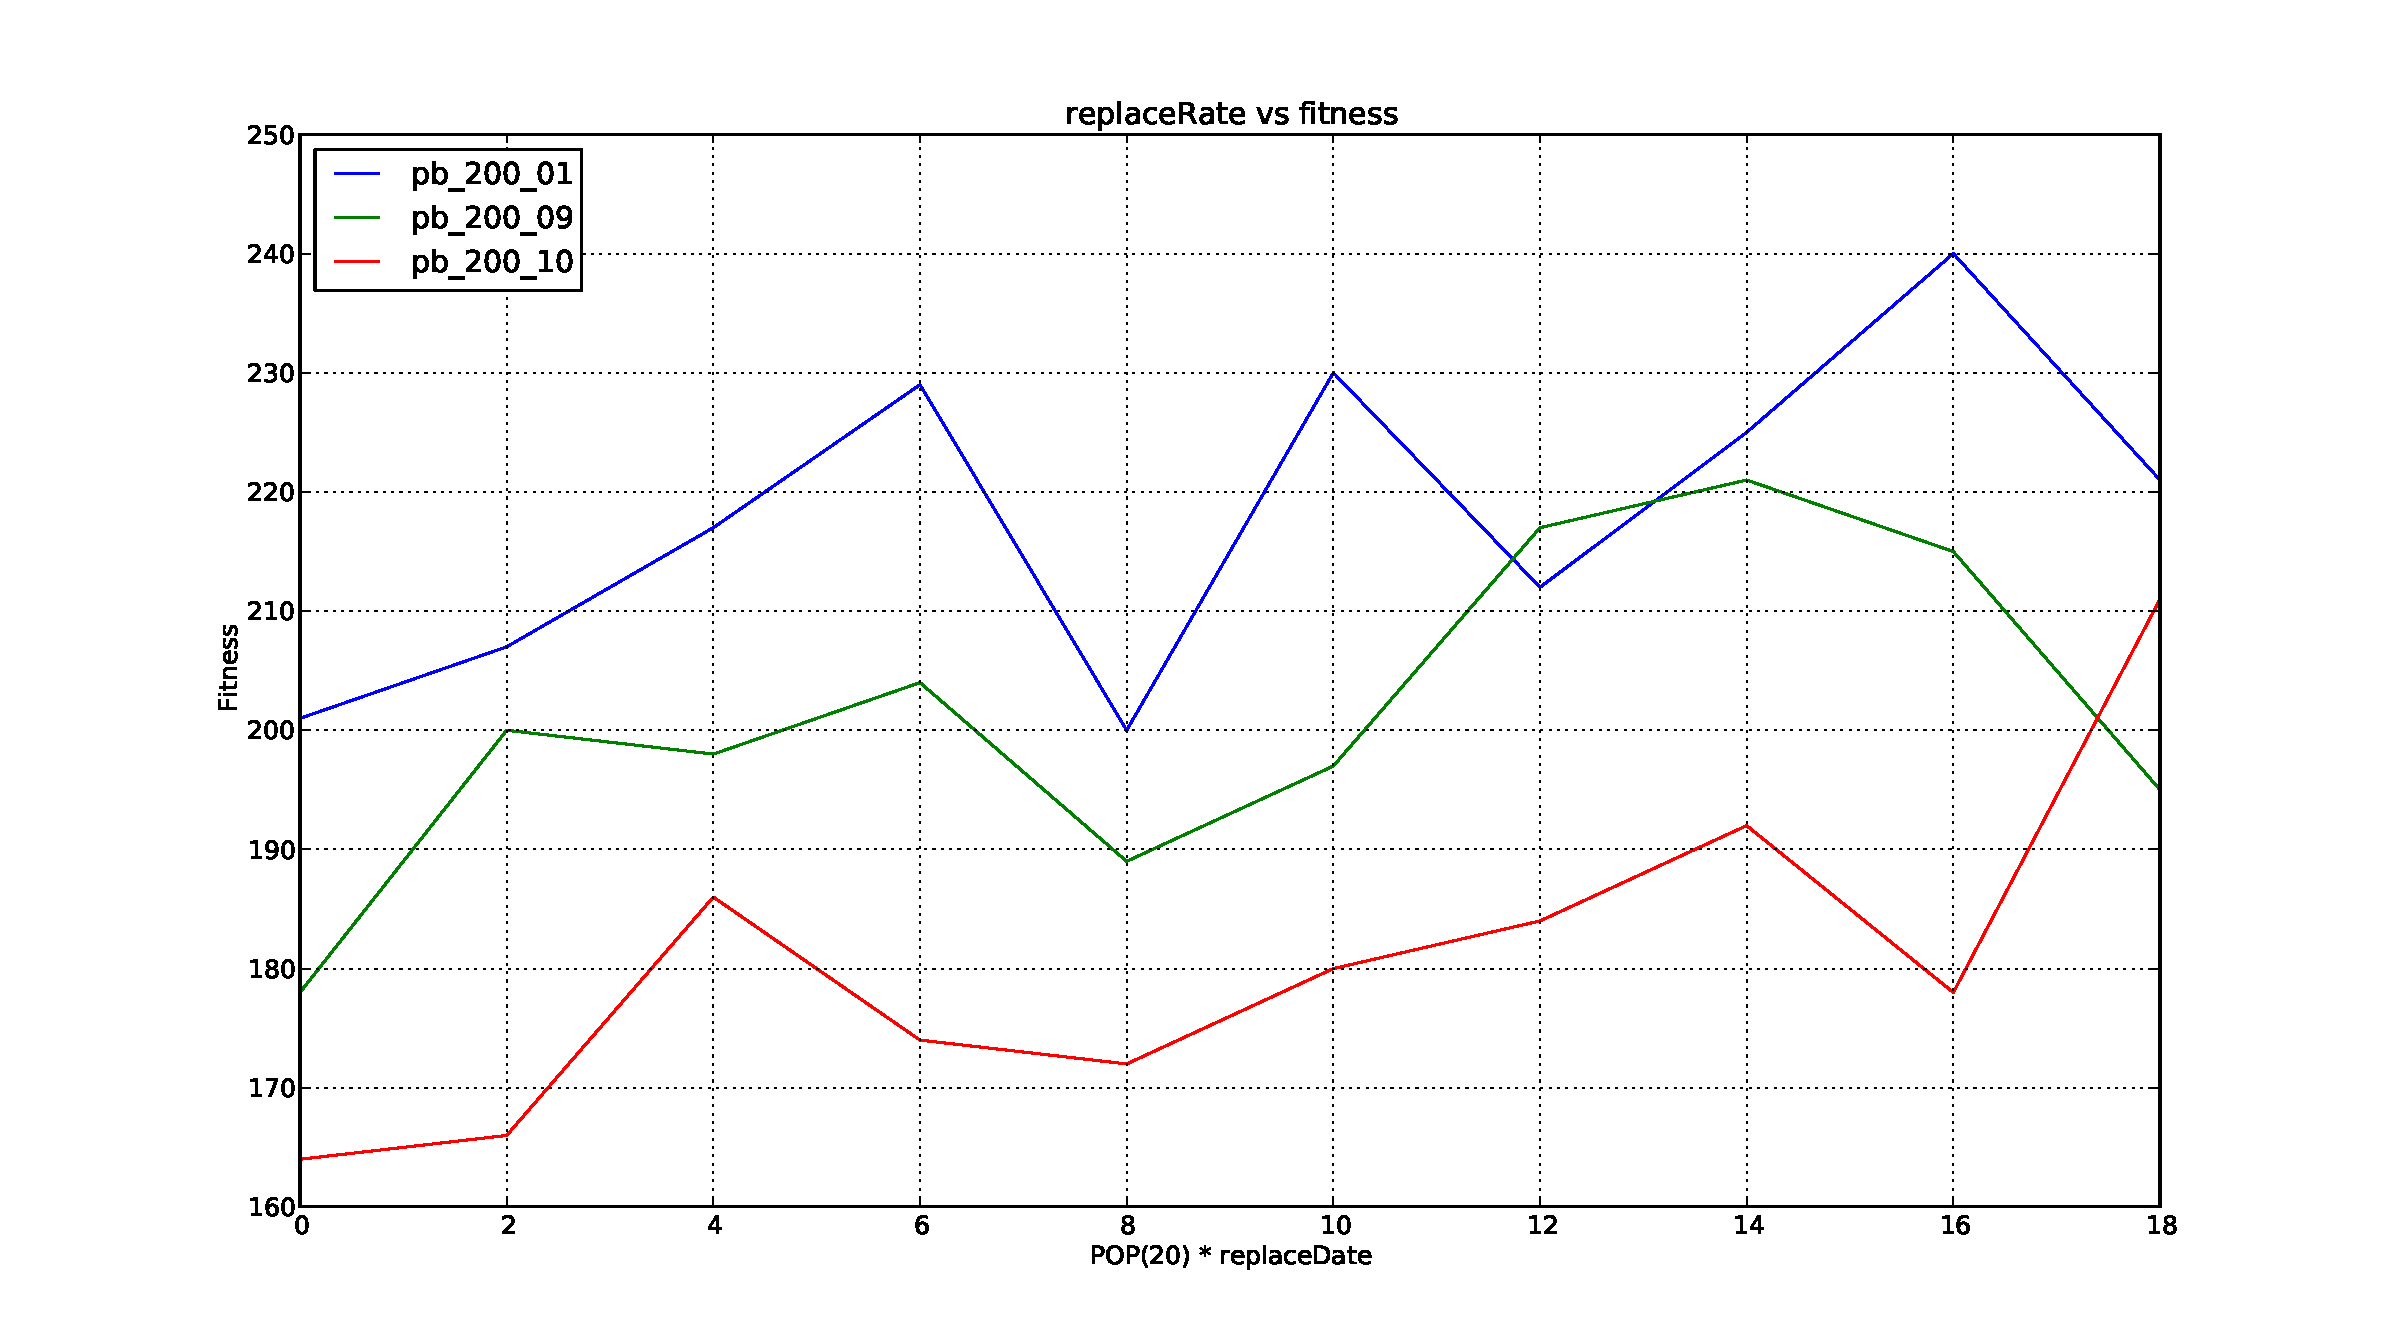
\includegraphics[width=0.95\textwidth]{img/3.pdf}
	\caption{Comparaci\'on de las tres instancias dado un cambio en la tasa de reemplazo}
	\label{fig:3}
\end{center}
\end{figure}

\textbf{Configuración escogida:}\\

\begin{center}
\begin{tabular}{|l|c|c|c|c|}
	\hline
	\textbf{Instancia} & \textbf{POP*replaceRate} & \textbf{Mejor resultado} & \textbf{Tiempo [s]} & \textbf{Tiempo total [s]}\\\hline
	\texttt{pb\_200\_01.txt} & 8 & 200 & 1.374 & 13.246 \\\hline
	\texttt{pb\_200\_09.txt} & 0 & 178 & 1.463 & 12.027 \\\hline
	\texttt{pb\_200\_10.txt} & 0 & 164 & 0.515 & 12.133   \\\hline
\end{tabular}
\end{center}


\newpage
\subsubsection{Factor de clonación y Tasa de clonación}

\textbf{Prueba}: \blue{prueba4} \\

\textbf{Parámetros involucrados}: Tasa de clonación y Factor de clonación. \\

\textbf{Objetivo}: Estudiar el efecto de la tasa y el factor de clonación en conjunto de acuerdo a fitness obtenido para la variación
de los dos parámetros en todo tu dominio.\\

\textbf{Metodología}: Se prueban varias combinaciones de valores para ver el efecto de los parámetros y poder observar su comportamiento.\\

\textbf{Configuración escogida:}\\

\begin{small}
\begin{center}
\begin{tabular}{|l|c|c|c|c|c|}
	\hline
	\textbf{Instancia} & \textbf{clonationRate} & \textbf{clonationFactor} &\textbf{Mejor resultado} & \textbf{Tiempo [s]} & \textbf{Tiempo total [s]}\\\hline
	\texttt{pb\_200\_01.txt} & 0.6 & 1   & 192 & 1.241 & 132.608 \\\hline
	\texttt{pb\_200\_09.txt} & 0.6 & 1   & 180 & 1.378 & 132.068 \\\hline
	\texttt{pb\_200\_10.txt} & 0.5 & 0.9 & 160 & 1.379 & 132.124 \\\hline
\end{tabular}
\end{center}
\end{small}
\normalsize
\textbf{Gráfico:}\\

\begin{figure}[h!]
\begin{center}
	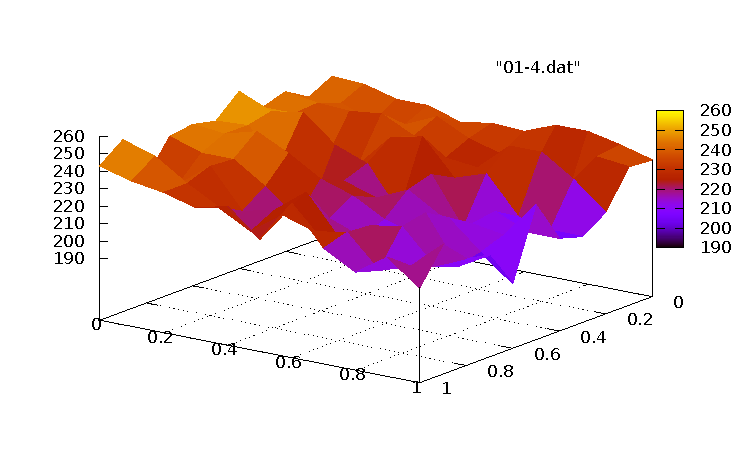
\includegraphics[width=0.95\textwidth]{img/01-4.pdf}
	\caption{Comparaci\'on de la instancia \texttt{pb\_200\_01.txt} variando \texttt{clonationRate} y \texttt{clonationFactor}}
	\label{fig:4-1}
\end{center}
\end{figure}

\begin{figure}[h!]
\begin{center}
	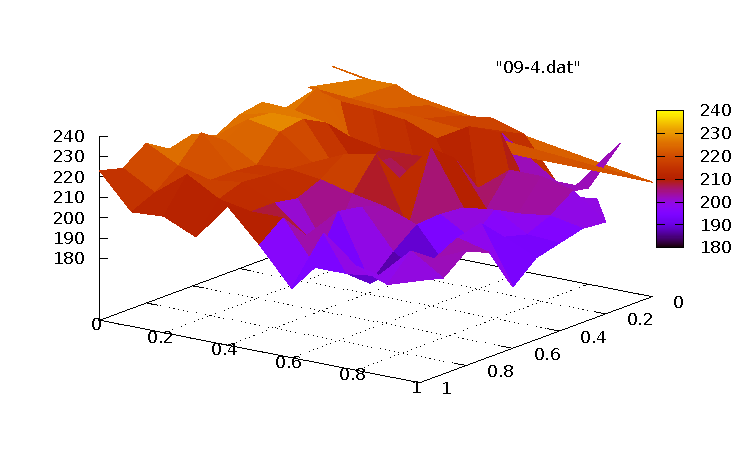
\includegraphics[width=0.95\textwidth]{img/09-4.pdf}
	\caption{Comparaci\'on de la instancia \texttt{pb\_200\_09.txt} variando \texttt{clonationRate} y \texttt{clonationFactor}}
	\label{fig:4-2}
\end{center}
\end{figure}

\newpage 
\begin{figure}[h!]
\begin{center}
	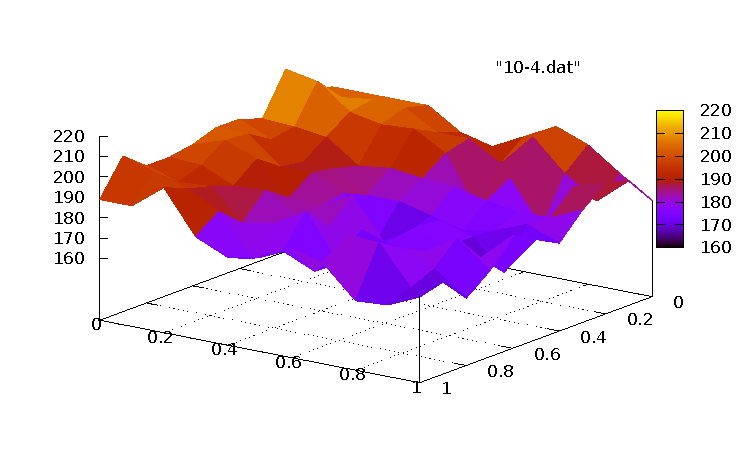
\includegraphics[width=0.95\textwidth]{img/10-4.pdf}
	\caption{Comparaci\'on de la instancia \texttt{pb\_200\_10.txt} variando \texttt{clonationRate} y \texttt{clonationFactor}}
	\label{fig:4-3}
\end{center}
\end{figure}


\newpage
%
%
%elegir una configuración para cada instancia
%	-indicar el fitness
%	-identificar claramente las características del algoritmo.
%	-estimación del tiempo en realizarla.
